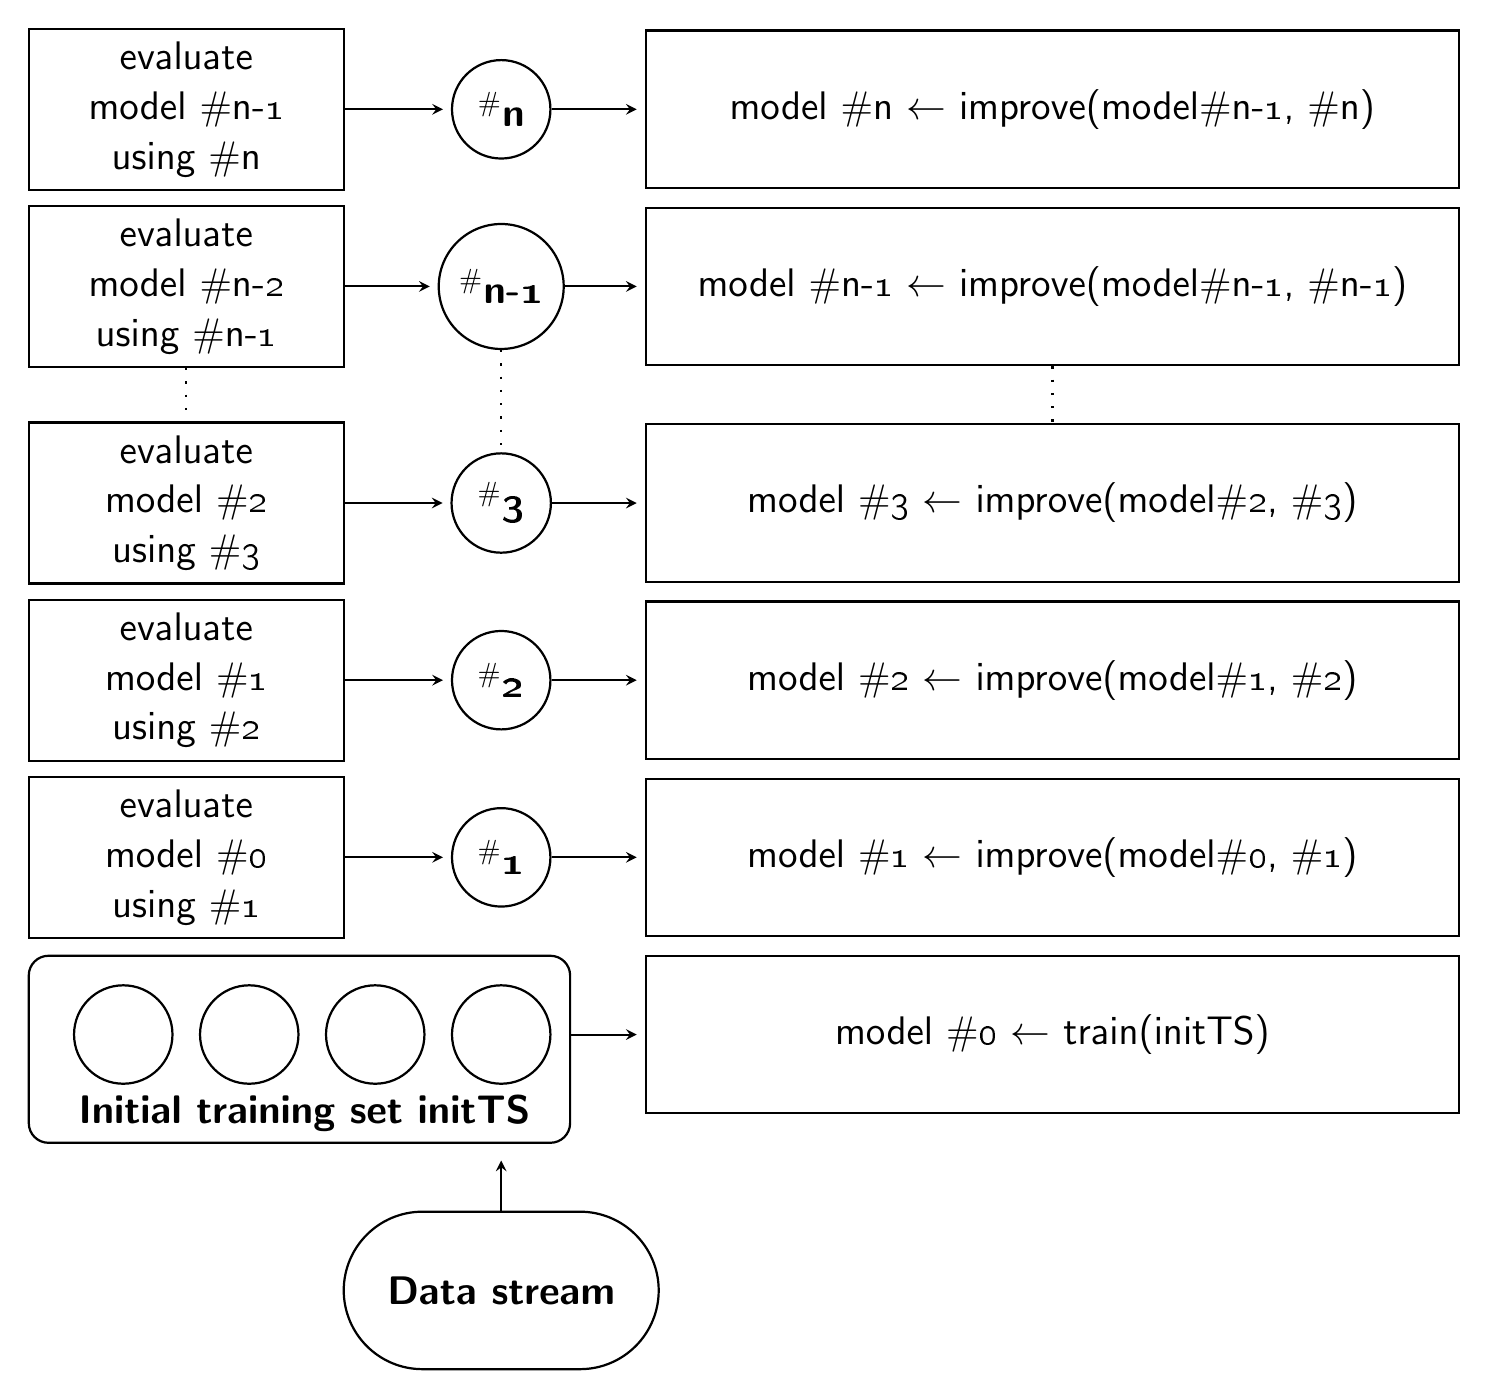
\begin{tikzpicture}[auto, thick, node distance=2cm, font=\sffamily]
\Large
\tikzset{%
	contra/.style = {black, fill = white, text=black},
	ds/.style = {draw,rectangle, minimum height = 2cm, minimum width = 4cm, rounded corners = 1cm, contra},
	chunk/.style = {draw,circle, minimum height = 1.25cm, minimum width = 1.25cm, contra},
	eval/.style = {draw,rectangle, minimum height = 2cm, minimum width = 4cm, text width=2.5cm, align = center},
	model/.style = {draw,rectangle, minimum height = 2cm, minimum width = 10cm, text width=10cm, align = center},
	con/.style = {->,shorten >=1mm,line width=.25mm,>=stealth}
}

% Data stream

\draw node at (0,-3) [chunk] (c1) {\bfseries $^\#$n}; 
\draw node at (0,-5.25) [chunk] (c2) {\bfseries $^\#$n-\oldstylenums1}; 
\draw node at (0,-8) [chunk] (c3) {\bfseries $^\#$\oldstylenums3}; 
\draw node at (0,-10.25) [chunk] (c4) {\bfseries $^\#$\oldstylenums2}; 
\draw node at (0,-12.5) [chunk] (c5) {\bfseries $^\#$\oldstylenums1};

\draw node at (-4,-3) [eval] (e1)
{evaluate model \#n-\oldstylenums1 \hspace{2em}using \#n}; 
\draw node at (-4,-5.25) [eval] (e2)
{evaluate model \#n-\oldstylenums2 \hspace{2em}using \#n-\oldstylenums1}; 
\draw node at (-4,-8) [eval] (e3)
{evaluate model \#\oldstylenums2 \hspace{2em}using \#\oldstylenums3}; 
\draw node at (-4,-10.25) [eval] (e4)
{evaluate model \#\oldstylenums1 \hspace{2em}using \#\oldstylenums2}; 
\draw node at (-4,-12.5) [eval] (e5)
{evaluate model \#\oldstylenums0 \hspace{2em}using \#\oldstylenums1}; 

\draw node at (7,-3) [model] (m1)
{model \#n $\leftarrow$ improve(model\#n-\oldstylenums1, \#n)};
\draw node at (7,-5.25) [model] (m2) 
{model \#n-\oldstylenums1 $\leftarrow$ improve(model\#n-\oldstylenums1, \#n-\oldstylenums1)};
\draw node at (7,-8) [model] (m3) 
{model \#\oldstylenums3 $\leftarrow$ improve(model\#\oldstylenums2, \#\oldstylenums3)};
\draw node at (7,-10.25) [model] (m4) 
{model \#\oldstylenums2 $\leftarrow$ improve(model\#\oldstylenums1, \#\oldstylenums2)};
\draw node at (7,-12.5) [model] (m5) 
{model \#\oldstylenums1 $\leftarrow$ improve(model\#\oldstylenums0, \#\oldstylenums1)};
\draw node at (7,-14.75) [model] (m6) 
{model \#\oldstylenums0 $\leftarrow$ train(initTS)};


\draw node at (-2.5,-15.75) {\bfseries Initial training set initTS};
\draw [rounded corners = .25cm] (-6,-13.75) rectangle (.875,-16.125);
\draw node at (-4.8,-14.75) [chunk] { };
\draw node at (-3.2,-14.75) [chunk] { }; 
\draw node at (-1.6,-14.75) [chunk] { }; 
\draw node at (0,-14.75) [chunk] { }; 

\draw node at (0,-18.0) [ds] (ds) {\bfseries Data stream};

\draw[con] (ds) -- (0,-16.25);
\draw[con] (e1) -- (c1);
\draw[con] (c1) -- (m1);
\draw[con] (e2) -- (c2);
\draw[con] (c2) -- (m2);
\draw[con] (e3) -- (c3);
\draw[con] (c3) -- (m3);
\draw[con] (e4) -- (c4);
\draw[con] (c4) -- (m4);
\draw[con] (e5) -- (c5);
\draw[con] (c5) -- (m5);
\draw[con] (.875,-14.75) -- (m6);

\draw[loosely dotted] (e2) -- (e3);
\draw[loosely dotted] (c2) -- (c3);
\draw[loosely dotted] (m2) -- (m3);

\end{tikzpicture}